\setcounter{secnumdepth}{1}
\section{Projektive Geometrie}
\setcounter{secnumdepth}{0}
$(P,G,I)$: $P$, $G$ Mengen, $I \subseteq P \times G$.

$P$: Menge der Punkte \\
$G$: Menge der Geraden \\
$I$: Inzidenzrelation.

Schreib- und Sprechweisen:
\begin{itemize}
 \item Statt $(p,g) \in I$ schreibe $pIg$, ``$p$ liegt auf $g$''. 
 \item Zwei Geraden $g_1$, $g_2$ ``schneiden sich in $p$'' heißt $pIg_1$ und $pIg_2$. 
 \item Drei Punkte $p_1$, $p_2$, $p_3$ heißen ``kollinear'', falls es $g \in G$ gibt, so dass $p_1$, $p_2$, $p_3$ auf $g$ liegen.
 \item Für $g_1, g_2 \in G$ ist
  \[ g_1 \cap g_2 = \begin{cases}
                   p, &\text{falls sich } g_1, g_2 \text{ in } p \text{ schneiden.} \\
                   \emptyset, &\text{falls sie sich nicht schneiden.} \\
                   g_1 = g_2, &\text{falls die Geraden zusammen fallen.}
                  \end{cases} \]
\end{itemize}

\subsection{Projektiver Raum}
\begin{defn*}\label{def:proj}
 Ein \emph{projektiver Raum} $\proj = (P,G,I)$ besteht aus zwei Mengen $P$, $G$ und einer Relation $I \subseteq P \times G$, sodass gilt:
 \begin{enumerate}[\hspace{.5cm}{A}1)]
  \item Durch je zwei (verschiedene) Punkte $p_1$, $p_2$ geht genau eine Gerade. Bezeichne diese Gerade mit $p_1 p_2$.
  \item Sind $p_1$, $p_2$, $p_3$, $p_4$ vier Punkte, sodass sich die Geraden $p_1 p_2$ und $p_3 p_4$ schneiden, dann treffen sich auch $p_1 p_3$ und $p_2 p_4$.
  \item Auf jeder Geraden liegen mindestens drei Punkte.
  \item Es gibt mindestens zwei Geraden.
 \end{enumerate}
\end{defn*}

\begin{defn*}
 Der projektive Raum $\proj = (P,G,I)$ heißt eine \emph{projektive Ebene}\footnote{Die Zeichenebene ist keine projektive Ebene! Zum Beispiel kann man in A2 $p_1$, $p_2$, $p_3$, $p_4$ so wählen, dass $p_1 p_3$ und $p_2 p_4$ parallel sind.}, falls die folgende Verschärfung von A2 gilt:
 \begin{enumerate}[\hspace{.5cm}{A}1)]
  \item [A2')] Je zwei Geraden schneiden sich.
 \end{enumerate}
\end{defn*}

\begin{bem}
 Aus A1 folgt: Falls Geraden $g_1$, $g_2$ mindestens zwei Punkte $p_1$, $p_2$ gemeinsam haben, dann folgt $g_1 = g_2$. Das heißt zwei (verschiedene) Geraden $g_1$, $g_2$ schneiden sich in höchstens einem Punkt.
\end{bem}

Erinnerung: In einem Schiefkörper $(K, +, \cdot)$ gelten alle Körperaxiome, bis auf die Kommutativität von $\cdot$. Also ist $(K, +)$ eine abelsche Gruppe (mit neutralem Element $0$) und $(K \setminus \{ 0 \}, \cdot)$ ist eine Gruppe (mit neutralem Element 1). Es gelten die Distributivgesetze:
\begin{align*}
 a(b+c) = ab + ac, \\
 (a+b)c = ac + bc.
\end{align*}

Im (Links-)Vektorraum $V$ über dem Schiefkörper $K$ gelten alle Axiome außer, dass der Skalarbereich ein Schiefkörper ist, zum Beispiel $\lambda( \mu x ) = (\lambda \mu) x$, $\lambda, \mu \in K$, $x \in V$.

Wenn man eine lineare Abbildung durch Matrizen beschreiben will, besser Rechtsvektorraum $A(x\lambda) = (Ax) \lambda$.

\begin{bem}
 Grundlegendes aus der linearen Algebra gilt auch für Vektorräume über Schiefkörpern (z.B. Basis, Dimension, Dimensionssatz). Determinanten sind nicht vernünf\-tig definierbar und alles was mit ihnen zusammenhängt gilt damit auch nur eingeschränkt.
\end{bem}

\begin{defn*}
 Ein \emph{echter Schiefkörper} $K$ ist ein Schiefkörper, bei dem die Multiplikation \emph{nicht} kommutativ ist.
\end{defn*}

Sei $K$ ein Schiefkörper, $V$ ein (Links-)$K$-Vektorraum. Definiere
\begin{itemize}
 \item $P := \{ Kx | x \in V \setminus \{ 0 \} \}$ Menge der 1-dimensionalen linearen Unterräume,
 \item $G := \{ Kx + Ky | x, y \in V $ linear unabhängig $\}$ Menge der 2-dimensionalen linearen Unterräume.
 \item $p I G \Leftrightarrow p \subseteq g$, $p$ liegt auf $g$, wenn falls der 1-dimensionale Unterraum $p$ in $g$ enthalten ist.
\end{itemize}

\begin{defn*}
 $\proj(V) := (P,G,I)$.
\end{defn*}

\begin{deno*}
 $[x] := Kx$ (für $x \in V \setminus \{ 0 \}$), $[x,y] := Kx + Ky$ ist die lineare Hülle von $x,y$.
\end{deno*}

\begin{thm}
 Falls $V$ ein $K$-Vektorraum über einem Schiefkörper $K$ mit $\dim V \ge 3$ ist, dann ist $\proj(V)$ ein projektiver Raum. Ist $\dim V = 3$, dann ist $\proj(V)$ eine projektive Ebene.
\end{thm}

\begin{proof}
 A1) Für $[x], [y] \in P$ mit $[x] \ne [y]$ gilt $x,y$ sind linear unabhängig und damit ist $[x,y]$ der einzige zweidimensionale Unterraum, der $[x]$ und $[y]$ enthält.
 
 A2) Seien $p_1 = [x_1]$, $p_2 = [x_2]$, $p_3 = [x_3]$, $p_4 = [x_4] \in P$ vier verschiedene Punkte, sodass sich $p_1 p_2 = [x_1, x_2]$ und $p_3 p_4 = [x_3, x_4]$ treffen. Dann ist $\dim ( [x_1 x_2] \cap [x_3 x_4] ) \ge 1$ und wir erhalten mit der Dimensionsformel:
 \begin{align*}
  \dim( [x_1, x_2, x_3, x_4]) &= \dim( [x_1, x_2] ) + \dim( [x_3, x_4] ) - \dim( [x_1,x_2] \cap [x_3,x_4] ) \\
  &\le 2+2-1 = 3.
 \end{align*}
 Nun benutzen wir nochmals die Dimensionsformel, um $\dim( [x_1,x_3] \cap [x_2,x_4] )$ abzuschätzen:
 \begin{align*}
  \dim( [x_1,x_3] \cap [x_2,x_4] ) &= \dim( [x_1, x_3] ) + \dim( [x_2, x_4] ) - \dim( [x_1, x_2, x_3, x_4]) \\
  &\ge 2 + 2 - 3 = 1.
 \end{align*}
 Also treffen sich auch $p_1 p_3$ und $p_2 p_4$.
 
 A3) Sei $[x,y] \in G$, also $\{ x,y \}$ linear unabhängig, dann sind auch $\{ x, x+y \}$ und $\{ y, x+y \}$ linear unabhängig, also $[x]$, $[y]$, $[x+y]$ drei verschiedene Punkte auf $[x,y]$.
 
 A4) Da $\dim V \ge 3$ gibt es linear unabhängige Vektoren $x,y,z \in V$. Damit ist $[x,y] \ne [y,z]$ (beide in $G$).
 
 A2') Falls $\dim V = 3$, $g_1, g_2 \in G$, $g_1 \ne g_2$, dann gilt 
 \[ \dim( g_1 \cap g_2 ) = \dim g_1 + \dim g_2 - \dim( g_1 + g_2 ) = 2 + 2 - 3 = 1. \qedhere \]
\end{proof}

\begin{defn*}
 Unter einem \emph{Dreieck} verstehen wir ein Tripel $(A_1, A_2, A_3)$ von nicht kollinearen Punkten. $A_1, A_2, A_3$ heißen die \emph{Ecken}, $A_2 A_3, A_1 A_3, A_1 A_2$ heißen die \emph{Seiten} des Dreiecks.
\end{defn*}

\subsection{Satz von Desargues}
\begin{defn*}
 Sei $\proj$ ein projektiver Raum. $\proj$ heißt \emph{desarguessch} (oder in $\proj$ gilt der Satz von Desargues), falls für je zwei Dreiecke $(A_1, A_2, A_3)$, $(B_1, B_2, B_3)$, bei denen die einander entsprechenden Ecken und Seiten verschieden sind, gilt: 
 \begin{addmargin}[.5cm]{0cm}
 Wenn die drei Verbindungsgeraden durch die einander entsprechenden Ecken durch einen Punkt gehen, dann sind die drei Schnittpunkte der einander entsprechenden Seiten kollinear. 
 \end{addmargin}
 Also:
 \begin{addmargin}[.5cm]{0cm}
 Falls es $Z \in P$ gibt mit $z = A_1 B_1 \cap A_2 B_2 \cap A_3 B_3$, dann sind
 \[ P_{12} := A_1 A_2 \cap B_1 B_2, \quad P_{13} := A_1 A_3 \cap B_1 B_3, \quad P_{23} := A_2 A_3 \cap B_2 B_3 \]
 kollinear.
 \end{addmargin}

 Falls die 10 Punkte $Z, A_1, A_2, A_3, B_1, B_2, B_3, P_{12}, P_{13}, P_{23}$ und 10 Geraden\footnote{Die sechs Seiten der Dreiecke, die drei Verbindungsgeraden und die Gerade, auf der $P_{12}, P_{13}, P_{23}$ liegen.}  paarweise verschieden sind, nennt man diese Konfiguration aus 10 Punkten und 10 Geraden die \emph{Konfiguration von Desargues}.
\end{defn*}

\begin{figure}[ht]
 \center
 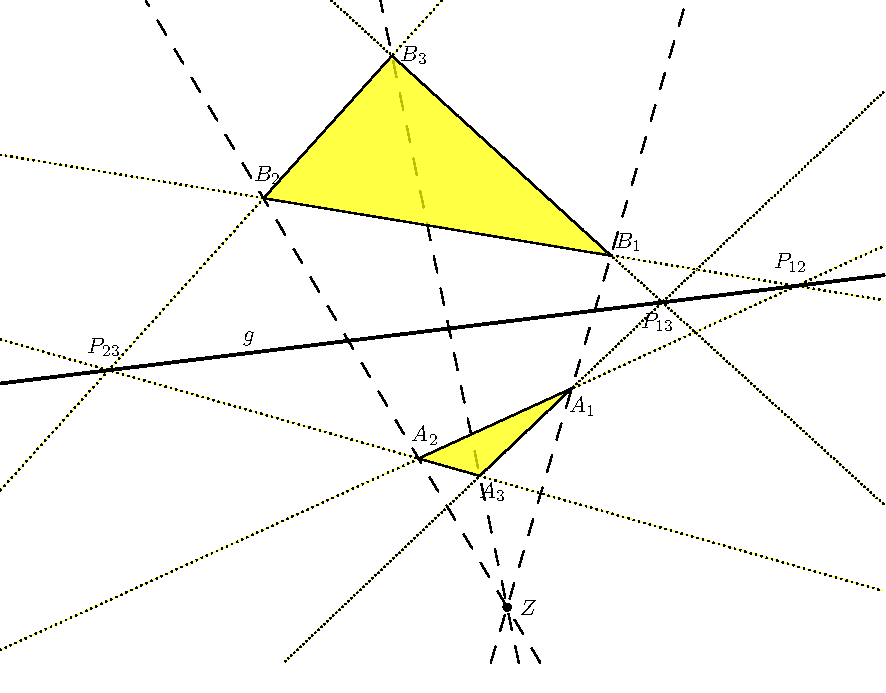
\includegraphics[width=12cm]{img/desargues}
\end{figure}

\begin{thm}
 Sei $V$ ein $K$-Vektorraum über einem Schiefkörper $K$ mit $\dim V \ge 3$. Dann ist $\proj(V)$ desarguessch.
\end{thm}

\begin{proof}
 Falls $Z$ mit einer Ecke übereinstimmt ist die Behauptung trivial. Sei also o.B.d.A. $Z \ne A_i$, $Z \ne B_i$, $A_i \ne B_i$ für $i = 1,2,3$. Seien $Z = [v]$, $A_i = [v_i]$. 
 
 Wir können nun $B_i = [v + v_i]$, $i = 1,2,3$ annehmen. Begründung: Wähle $v$ fest und $\tilde{v}_i$ mit $[\tilde{v}_i] = A_i$. Dann sind $B_i = [\lambda_i v + \mu_i \tilde{v}_i]$ für gewisse $\lambda_i, \mu_i \in K$. Es gilt $\lambda_i \ne 0$ weil $B_i \ne Z$ und $\mu_i \ne 0$ weil $B_i \ne A_i$. Also gilt 
 \[ B_i = \lambda_i^{-1} [\lambda_i v + \mu_i \tilde{v}_i] = [v + \underbrace{\lambda_i^{-1} \mu_i \tilde{v}_i}_{=: v_i}] = [v + v_i], \]
 $A = [v_i]$ weil $[\tilde{v_i}] = [v_i]$. Damit folgt 
 \[ P_{12} = A_1 A_2 \cap B_1 B_2 = [v_1 , v_2] \cap [v + v_1, v + v_2 ] = [v_1 - v_2], \]
 denn die projektiven Geraden $A_1 A_2$ und $B_1 B_2$ sind nach Voraussetzung verschieden, also
 \[ \dim( [v_1, v_2] \cap [v + v_1, v + v_2 ] ) = 2 + 2 - \dim[v_1, v_2, v] = 1 \]
 und $v_1 - v_2 \in [v_1, v_2] \cap [v + v_1, v + v_2]$, der Punkt $v_1-v_2$ liegt sowohl in der linearen Hülle von $(v_1, v_2)$ als auch in $(v + v_1, v + v_2)$.

 Entsprechend folgen $P_{23} = [v_2 - v_3]$, $P_{13} = [v_1 - v_3]$. Also liegen $P_{12}$, $P_{13}$, $P_{23}$ auf der projektiven Geraden $[v_1 - v_2, v_2 - v_3]$. Damit gilt in $\proj(V)$ der Satz von Desargues.
\end{proof}

\subsection{Satz von Pappos}
\begin{defn*}
 Sei $\proj$ ein projektiver Raum. In $\proj$ \emph{gilt der Satz von Pappos}\footnote{Pappos von Alexandria, ca. 300}, falls für je 7 verschiedene Punkte $Z, A_1, A_2, A_3, B_1, B_2, B_3$ gilt:
 \begin{addmargin}[.5cm]{0cm} 
 Falls $Z, A_1, A_2, A_3$ auf einer Geraden $g$ liegen und $Z, B_1, B_2, B_3$ auf einer Geraden $h \ne g$ liegen, dann sind die Punkte 
 \[ P_{12} := A_1 B_2 \cap A_2 B_1, \quad P_{23} := A_2 B_3 \cap A_3 B_2, \quad P_{13} := A_1 B_3 \cap A_3 B_1 \]
 kollinear.
 \end{addmargin}
\end{defn*}

\newpage

\begin{figure*}[ht]
 \center
 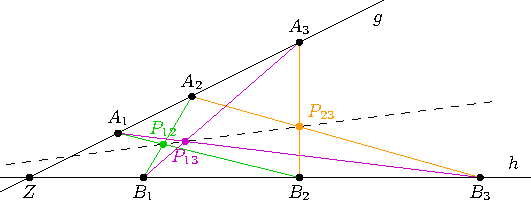
\includegraphics[width=12cm]{img/pappos}
\end{figure*}

\begin{thm}
 Sei $V$ ein $K$-Vektorraum über einem Schiefkörper $K$ und $\dim V \ge 3$. Dann gilt in $\proj(V)$ der Satz von Pappos genau dann, wenn $K$ kommutativ, also ein Körper ist.
\end{thm}

\begin{proof}
 Seien 
 \[ \begin{aligned}
     Z   &:= g \cap h = [u], \\
     A_1 &:= [v] \text{ und o.B.d.A. } A_2 = [u + v] \text{ (ersetze ggf. $v$ durch ein geeignetes $\lambda v$)}, \\
     B_1 &:= [w] \text{ und o.B.d.A. } B_2 = [u + w].
    \end{aligned} \]
 $u, v, w$ sind linear unabhängig, da $g \ne h$. Dann ist $P_{12} = A_1 B_2 \cap A_2 B_1 = [u + v + w]$. 
 
 ``$\Leftarrow$'' Sei $K$ ein Körper. Zu zeigen: $P_{12}, P_{13}, P_{23}$ sind kollinear.
 
 Für $A_3, B_3$ gibt es $r, s \in K$ mit $A_3 = [ru+v]$, $B_3 = [su+w]$. Dann ist 
 \[ P_{13} = A_3 B_1 \cap A_1 B_3 = [ru + v, w] \cap [v, su + w] = [rsu+sv+rw] =: [v_{13}], \]
 denn $s(ru+v) + rw = rsu + sv + rw = sv + r(su + w)$. Dabei gilt $rs = sr$, weil $K$ kommutativ ist.
 \[ P_{23} = A_2 B_3 \cap A_3 B_2 = [u+v, su + w] \cap [ru + v, u+w] \]
 und es gilt
 \[ \begin{aligned}
    (rs-1)u + (s-1)v + (r-1)w 
    &= (s-1) (u+v) + (r-1)(su +w) \\
    &= (s-1)(u+w) + (s-1)(ru+v),
    \end{aligned} \]
 also folgt
 \[ P_{23} = [ (rs-1)u + (s-1)v + (r-1)w ] =: [v_{23}]. \]
 Wir sehen nun $v_{13} - v_{23} = u + v + w$, also ist $P_{12} \in P_{13} P_{23}$ und damit sind die Punkte kollinear.
 
 ``$\Rightarrow$'' Gelte der Satz von Pappos. Zu zeigen: $K$ ist ein Körper, also $rs = sr$ für $r,s \in K$.
 
 Seien o.B.d.A.\footnote{Wir schließen 0 und 1 aus, da sie mit allen Elementen von $K$ kommutieren.} $r,s \in K \setminus \{ 0, 1 \}$, $A_3 := [ru+v]$, $B_3 := [su+v]$. Dann gibt es $x,y \in V$ mit $[x+y] = [u + v + w]$.
 
 Seien $P_{13} = [x]$, $P_{23} = [y]$, dann gibt es wegen des Satzes von Pappos $t_1, \ldots, t_8 \in K$, so dass
 \begin{align*}
    x &=   &   t_1 v + t_2 (su+w) &= t_3 w + t_4 (ru+v) \tag{1} \\
    y &=   &   t_5 (u+v) + t_6 (su+w) &= t_7 (u+w) + t_8 (ru+v) \tag{2} \\
  x+y &=   &   u+v+w &= t_1 v + t_2 (su+w) + t_5 (u+v) + t_6 (su+w) \tag{3}
 \end{align*}
 Weil $u,v,w$ linear unabhängig sind, folgt aus (3)
 \[ \left. \begin{aligned}
    w: \quad 1 &= t_2 + t_6 \\
    u: \quad 1 &= (t_2+t_6) s + t_5 = s + t_5 \\
    v: \quad 1 &= t_1 + t_5
    \end{aligned}
    \quad \right\} \Rightarrow 
    \begin{aligned}
     t_1 &= s, \\
     t_2 &= 1 - t_6, \\
     t_5 &= 1 - s. 
    \end{aligned} \]
 Zusammen mit (1) folgt
 \[ v: \quad t_4 = t_1 = s, \qquad u: \quad t_2 s = t_4 r, \qquad w: \quad t_2 = t_3. \]
 Mit $t_2 = 1 - t_6$ aus (3) gilt also
 \[ (1-t_6)s = t_2 s = t_4 r = sr \qRq t_6 s = s - sr \qRq t_6 = 1 - srs^{-1}. \tag{$\circ$} \]
 Zusammen mit (2) folgt
 \[ u: \quad t_5 + t_6s = t_7 + t_8 r, \qquad v: \quad t_8 = t_5, \qquad w: \quad t_7 = t_6. \]
 Nun setzen wir ($\circ$) und $t_5 = 1-s$ ein:
 \begin{align*}
     t_5 + t_6 s = t_6 + t_5 r \quad
     &\Rightarrow & (1-s) + (s-sr) &= (1 - srs^{-1}) + (1-s)r \\
     &\Rightarrow & -srs^{-1} + r &= 0 \\
     &\Rightarrow & srs^{-1} &= r \\
     &\Rightarrow & rs &= sr. \qedhere 
 \end{align*}
\end{proof}

\begin{bem}
 Aus dem Beweis des Satzes folgt in $\proj(V)$ ($V$ ist ein $K$-Vektorraum mit $\dim V \ge 3$): $K$ kommutativ $\Leftrightarrow$ Es existieren paarweise verschiedene $Z, A_1, A_2, B_1, B_2 \in \proj(V)$ mit $Z = A_1 A_2 \cap B_1 B_2$. Für alle $A_3$ auf $A_1 A_2$ mit $A_3 \ne A_1, A_2$ und $B_3$ auf $B_1 B_2$ mit $B_3 \ne B_1, B_2$ gilt: $P_{ij} = A_i B_j \cap A_j B_i$, $i \ne j$ sind kollinear.
 
 Das heißt im Satz von Pappos kann man $Z, A_1, A_2, B_1, B_2$ fest wählen.
\end{bem}

\begin{deno*}
 Der Vektor $x \ne 0$ aus $K^n$ heißt \emph{homogene Koordinaten} von $[x] \in \proj(V)$. Falls $x \in K^n$ mit $x_n \ne 0$, dann ist
 \[ \left[ \begin{pmatrix} x_1 \\ \vdots \\ x_{n-1} \\ x_n \end{pmatrix} \right] =
    \left[ \begin{pmatrix} x_n^{-1} x_1 \\ \vdots \\ x_n^{-1} x_{n-1} \\ 1 \end{pmatrix} \right]. \]
\end{deno*}

Für $V = \real^n$ ist
\[ [x] = \left[ \frac{x}{\|x\|} \right] = \left[ \frac{-x}{\|x\|} \right]. \]
Der projektive Raum $\proj(\real^n)$ kann daher mit der $S^{n-1} \subseteq \real^n$ nach Identifikation von Antipodenpaaren identifiziert werden.
 
$S^{n-1}$ ist die Einheitssphäre. $x \in S^{n-1}$ heißt $x \in \real^n$, $\| x \| = 1$. Wir betrachten also statt Geraden die äquivalenten (gegenüberliegenden) Punkte der Einheitssphäre $S^{n-1}_\pm$, das heißt $x \sim x' \Leftrightarrow x = x'$ oder $x = -x'$.

\subsection{Dualität für projektive Ebenen}
\begin{thm}
 Sei $\proj = (P,G,I)$ eine projektive Ebene. Dann ist auch $\proj^* := (G,P,I^{-1})$ mit $I^{-1} := \{ (g,p) : (p,g) \in I \}$ eine projektive Ebene.
\end{thm}

$\proj^*$ ist die zu $\proj$ \emph{duale Ebene}. Offensichtlich gilt $\proj^{**} = \proj$.

\begin{proof}
 Zu zeigen: $\proj^*$ erfüllt die Axiome der projektiven Ebene A1), A2'), A3) und A4) (siehe S. \pageref{def:proj}).
 \begin{enumerate}[\hspace{.5cm}A2)]
  \item[A1)] Durch je zwei (verschiedene) Punkte $p_1$, $p_2$ geht genau eine Gerade.
  \item[A2')] Je zwei Geraden schneiden sich.
  \item[A3)] Auf jeder Geraden liegen mindestens drei Punkte.
  \item[A4)] Es gibt mindestens zwei Geraden.
 \end{enumerate}
 
 Die zu einer Aussage über $(P,G,I)$ duale Aussage ist die entsprechende Aussage für $(G,P,I^{-1})$\footnotemark.
 \footnotetext{Vertausche die Rollen von Punkten und Geraden und $I$ mit $I^{-1}$. Begriffe werden analog dualisiert, zum Beispiel die Gerade $P_1 P_2$ entspricht dem Punkt $g_1 \cap g_2$. Kollineare Punkte entsprechen kopunktalen Geraden.}
 
 Aus A1) und A2') folgt die Aussage:
 \begin{enumerate}[\hspace{.5cm}A2)]
  \item [$\widetilde{\text{A2}}$')] Je zwei Geraden schneiden sich in genau einem Punkt.
 \end{enumerate}

 Für die ersten beiden dualen Axiome folgt:
 \begin{enumerate}[\hspace{.5cm}{A}1 {dual})]
  \item[A1 dual)] ist offenbar dieselbe Aussage wie $\widetilde{\text{A2}}$').
  \item[A2' dual)] ist dieselbe Aussage wie A1).
 \end{enumerate}

 Die zu A3) und A4) dualen Aussagen sind
 \begin{enumerate}[\hspace{.5cm}{A}1 {dual})]
  \item[A3 dual)] Durch jeden Punkt gehen mindestens drei Geraden.
  \item[A4 dual)] Es gibt mindestens zwei Punkte.
 \end{enumerate}
 Aus A3) und A4) folgt offenbar A4 dual). 
 
 Zu zeigen: In $\proj$ gilt A3 dual). Sei $P$ ein Punkt. Dann gibt es nach A1) eine Gerade $g$ durch $P$.  Auf dieser liegen nach A3) mindestens zwei weitere Punkte $P_1$ und $P_2$. Nach A4) gibt es mindestens eine weitere Gerade $h$ und nach A2') schneiden sich $g$ und $h$ in einem Punkt $X$. Auf $h$ gibt es nach A3) zwei Punkte $Q_1, Q_2 \ne X$. Die Geraden $PQ_1, PQ_2$ und $PP_1$ sind paarweise verschieden. Damit gibt es mindestens drei Geraden durch $P$.
\end{proof}

\textbf{Dualitätsprinzip.} Wenn eine Aussage für alle projektiven Ebenen gilt, dann gilt auch die duale Aussage für alle projektiven Ebenen\footnote{Vertausche zum Beweis einfach $\proj$ mit $\proj^*$.}.

\begin{exmp*}
 Dualisiere die Aussage ``$\proj = (P,G,I)$ ist desarguessch.'' Beweise: Wenn $\proj$ desarguessch ist, dann ist es auch $\proj^*$.
 
 \begin{addmargin}[.5cm]{0cm} 
 \textbf{Aussage von Desargues.} Für alle $A_1, A_2, A_3, B_1, B_2, B_3 \in P$ mit $A_i \ne B_i$, sodass $A_1, A_2, A_3$ nicht kollinear sind und $B_1, B_2, B_3$ nicht kollinear sind, gilt: Falls $Z$ der Schnittpunkt von $A_1 B_1$, $A_2 B_2$ und $A_3 B_3$ ist, dann sind 
 \begin{align*}
  P_{12} &:= A_1 A_2 \cap B_1 B_2, \\
  P_{23} &:= A_2 A_3 \cap B_1 B_2, \\
  P_{13} &:= A_3 A_1 \cap B_3 B_1 
 \end{align*}
 kollinear.
 
 \textbf{Duale Aussage.} Für alle $g_1, g_2, g_3, h_1, h_2, h_3 \in G$ mit $g_i \ne h_i$, sodass $g_1, g_2, g_3$ nicht kopunktal\footnote{Das heißt, dass die drei Geraden sich nicht in \emph{einem} Punkt schneiden, sondern ein Dreieck bilden.} und $h_1, h_2, h_3$ nicht kopunktal sind, gilt: Falls $f$ eine Gerade durch $g_1 \cap h_1$, $g_2 \cap h_2$, $g_3 \cap h_3$ ist, dann sind
 \begin{align*}
  l_{12} &:= (g_1 \cap g_2)(h_1 \cap h_2), \\
  l_{23} &:= (g_2 \cap g_3)(h_2 \cap h_3), \\
  l_{31} &:= (g_3 \cap g_1)(h_3 \cap h_1 )
 \end{align*}
 kopunktal.
 \end{addmargin}
\end{exmp*}

\setcounter{thm}{5}
\begin{thm}
 Eine projektive Ebene $\proj$ ist desarguessch $\Leftrightarrow$ $\proj^*$ ist desarguessch.
\end{thm}

\subsection{Endliche projektive Räume}

\begin{defn*}
 Ein projektiver Raum $\proj = (P,G,I)$ heißt \emph{endlich}, falls $P$ endlich ist.
\end{defn*}

\begin{deno*}
 Sei $g \in G$, dann bezeichnet $(g) := \{ p \in P : (p,g) \in I \}$ die Menge der Punkte auf der Geraden $g$.
\end{deno*}

\begin{thm*}[Hessenberg]
 Sei $\proj$ ein projektiver Raum, in dem der Satz von Pappos gilt. Dann gilt auch der Satz von Desargues.
\end{thm*}

Beweis nicht in der Vorlesung, siehe zum Beispiel
\begin{itemize}
 \item H. Lenz: Vorlesungen über projektive Geometrie,
 \item R. Lingenberg: Grundlagen der Geometrie I.
\end{itemize}

Beispiel für eine nichtdesarguessche projektive Ebene (siehe auch Übung): Moulton-Ebene.

\begin{lem}
 Sei $\proj$ ein projektiver Raum, $g_1, g_2 \in G$. Dann gibt es eine bijektive Abbildung $\varphi:(g_1) \to (g_2)$.
\end{lem}

\begin{proof}
 Sei O.B.d.A. $g_1 \ne g_2$. Wir unterscheiden zwei Fälle:
 \begin{enumerate}
  \item $(g_1) \cap (g_2) = \{ s \} \ne \emptyset$. Seien $P_1 \in (g_1)$, $P_2 \in (g_2)$ mit $P_1 \ne P_2 \ne S$ (diese existieren nach A3)). Nach A3) gibt es auch $P$ mit $P \ne P_1$, $P \ne P_2$ auf $P_1 P_2$. Es ist offenbar $P \notin (g_1)$ und $P \notin (g_2)$. Nach A2) schneidet eine Gerade $Px$ mit $x \in (g_1)$, $x \ne S$ die Gerade $g_2$ in einem eindeutig bestimmten Punkt $\pi(x) \ne S$. Die Gerade $PS$ schneidet $g_2$ nur in $S$. Definiere $pi:(g_1) \to (g_2)$ mit $\pi( x ) = xP \cap g_2$. $\pi$ ist offenbar bijektiv.
  \item $(g_1) \cap (g_2) ) \emptyset$. Wähle  auf $g_1$, $g_2$ Punkte $P_1 \in (g_1)$, $P_2 \in (g_2)$. Sei $h := P_1 P_2$. Dann gibt es nach dem 1. Fall bijektive Abbildungen $\pi_1: (g_1) \to (h)$ und $\pi_2: (h) \to (g_2)$. Also ist $\pi_2 \circ \pi_1: (g_1) \to (g_2)$ bijektiv. \qedhere
 \end{enumerate}
\end{proof}

\begin{figure*}[ht]
 \center
 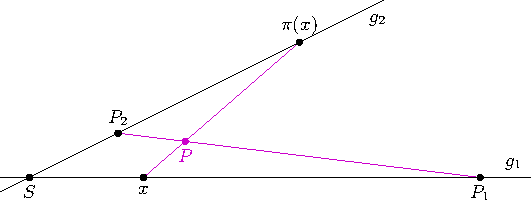
\includegraphics[width=12cm]{img/lemma27}
\end{figure*}

In einem endlichen projektiven Raum $\proj$ liegen also auf jeder Geraden gleich viele Punkte.

\begin{defn*}
 Ein endlicher projektiver Raum $\proj$ hat die \emph{Ordnung $q$}, wenn auf jeder Geraden $q+1$ Punkte liegen.
\end{defn*}

\begin{thm*}[Wedderburn]
 Jeder endliche Schiefkörper ist ein Körper.
\end{thm*}

\begin{thm}
 Sei $\proj = (P,G,I)$ eine projektive Ebene der Ordnung $q$. Dann gilt $|P| = |Q| = q^2 + q +1$. Auf jeder Geraden liegen $q+1$ Punkte und durch jeden Punkt gehen $q+1$ Geraden.
\end{thm}

\begin{proof}
 Nach Lemma 2.7 und Definition liegen auf jeder Geraden genau $q+1$ Punkte. Sei $p \in P$, $g \in G$ mit $p \notin (g)$. Jede Gerade durch $p$ schneidet $(g)$ in genau einem Punkt und durch jeden Punkt $p_1 \in (g)$ gibt es die Gerade $p p_1$. Damit haben wir eine Bijektion zwischen der Menge der Geraden durch $p$ und der Menge der Punkte auf $g$ definiert. Also gehen durch jeden Punkt $p$ genau $q++1$ Geraden. Damit gibt es genau 
 \[ \text{(Geraden durch $p$)} \cdot \text{(Punkte $\ne p$ auf $g$ durch $p$)} + \text{Punkt $p$} = (q+1)q + 1 = q^2 + q +1 \]
 Punkte. Dies ist auch gleich der Anzahl der Geraden, da $\proj^* = (G,P,I^{-1})$ auch eine projektive Ebene der Ordnung $q$ ist.
\end{proof}

\subsubsection*{Endliche Körper}
\begin{defn*}
 Sei $K$ ein Körper. Die \emph{Charakteristik} von $K$ ist definiert als
 \[ \chr K = \begin{cases} 
    p, &\text{falls $p \in \nat$ die kleinste Zahl mit $1 + 1 + \ldots + 1 = 0$ ist.} \\
    0, &\text{falls es keine solche Zahl gibt.}         
   \end{cases} \]
Falls $\chr K \ne 0$, dann ist $\chr K$ eine Primzahl, denn anderenfalls wäre $p = nm$ mit $1 < n < p$ und $1 < m < p$, also
\[ \underbrace{( 1 + 1 + \ldots + 1)}_n \cdot \underbrace{( 1 + 1 + \ldots + 1)}_m = 0 \]
\end{defn*}

\begin{exmp*}
 $\integer_p$ ist für eine Primzahl $p$ ein Körper der Charakteristik $p$.  
\end{exmp*}

Falls $K$ ein endlicher Körper ist, dann ist $\chr(K) = p \ne 0$ eine Primzahl. In $K$ betrachte die Menge
\[ P := \{ 0, 1, 1+1, \ldots, (p-1) \cdot 1 \} \subseteq K. \]
Dies ist ein Unterkörper von $K$ und $K$ ist ein $P$-Vektorraum, $\dim K = n \ne \infty$. $K$ hat genau $p^n$ Elemente. Also ist $(K,+) \simeq \integer_p^n$.

Es gilt $(K \setminus \{ 0 \}, \cdot ) \simeq \integer_{q-1}$, wobei $q = p^n = |K|$, das heißt es gibt $a \in K$ mit
\[ K^* := K \setminus \{ 0 \} = \{ 1, a, a^2, a^3, \ldots, a^{q-2} \}. \]
Also ist jedes Element von $K$ Nullstelle des Polynoms $x^q - x \in K[x]$. 

Die Abbildung $\varphi: K \to K$ mit $\varphi(x) = x^p$ ist ein Körperautomorphismus von $K$, denn
\begin{align*}
 \varphi(xy) &= (xy)^p = \varphi(x) \varphi(y) \\
 \varphi(x+y) &= (x+y)^p = \sum_{\nu = 0}^p \begin{pmatrix} p \\ \nu \end{pmatrix} x^\nu y^{p-\nu} \overset{\footnotemark}{=} x^p + y^p = \varphi(x) + \varphi(y)
\end{align*}
\footnotetext{Denn $\begin{pmatrix} p \\ \nu \end{pmatrix}$ ist  in $K$ für $1 \le \nu \le p-1$ durch $p$ teilbar, also $\begin{pmatrix} p \\ \nu \end{pmatrix} = 0$.}

$\varphi$ ist bijektiv, denn $\varphi^n = \id$,  $x^{p^n} = x^q = x$.

\begin{thm*}
 Sei $p$ eine Primzahl und $n \in \nat$. Dann gibt es bis auf Isomorphie genau einen Körper mit $q=p^n$ Elementen. Er ist der ``kleinste'' Körper, in dem das Polynom $x^q - x \in P[x]$ in Linearfaktoren zerfällt\footnote{Der ``Zerfällungskörper'' von $x^q - x$ über $P$.}.
 
 Die Unterkörper von $K$ mit $q = p^n$ sind genau die Körper der Form 
 \[ \{ x \in K | x^{p^i} = x \} = \{ 0 \} \cup \{ a^{k p^{n-i}} : k = 0, 1, \ldots, p^i -1 \},\]
 wobei $i \ge 1$ ein Teiler von $n$ ist. Also gibt es zu jedem $i \ge 1$ mit $i|n$ ($i$ teilt $n$) genau einen Unterkörper von $K$ mit $p^n$ Elementen und diese sind alle Unterkörper von $K$.
\end{thm*}

\subsubsection*{Konstruktion eines Körpers mit \texorpdfstring{$p^n$}{p hoch n} Elementen}
Wähle ein irreduzibles\footnote{Irreduzibel heißt, dass es \emph{keine} Polynome $p_1, p_2$ kleineren Grades gibt, sodass $p_0 = p_1 p_2$.} Polynom $n$-ten Grades $p_0(x) \in \integer_p[x]$. Dann ist $\integer_p[x] / (p_0)$ ein Körper mit $p^n$ Elementen.

Erzeugtes Ideal
\[ \{ p_0 f | f \in \integer_p[x] \} \]

\begin{defn*}\label{def:kollineation}
 Sei $\proj = (P,G,I)$, $\proj' = (P',G',I')$ projektive Räume. Eine \emph{Kollineation} $\alpha: \proj \to \proj'$ ist ein Paar $\alpha = (\alpha_1, \alpha_2)$ von bijektiven Abbildungen $\alpha_1:P \to P'$, $\alpha_2: G \to G'$, sodass $(p,g) \in I \Leftrightarrow (\alpha_1(p), \alpha_2(g) ) \in I'$ für alle $p \in P$, $g \in G$. 
 
 $\proj=(P,G,I)$ und $\proj' = (P', G', I')$ heißen \emph{isomorph} (geschrieben $\proj \simeq \proj'$), wenn es eine Kollineation $\alpha: \proj \to \proj'$ gibt.
 
 Schreibweise: Wir schreiben $\alpha(p), \alpha(g)$ statt $\alpha_1(p), \alpha_2(g)$, falls keine Missverständnisse zu befürchten sind.
\end{defn*}

\begin{bem}
 Die Menge der Kollineationen $\alpha: \proj \to \proj'$ ist mit $\circ$ eine Gruppe.
\end{bem}

\begin{thm*}[Koordinatisierungssatz]
 Sei $\proj = (P,G,I)$ ein desarguesscher projektiver Raum. Dann gibt es einen Schiefkörper $K$ mit einem $K$-Vektorraum $V$ mit $\dim V \ge 3$, sodass $\proj \simeq \proj(V)$ gilt.
\end{thm*}

\subsubsection*{Desarguessche endliche projektive Ebenen}
Sei $\proj$ eine endliche desarguessche projektive Ebene. Nach dem Koordinatisierungssatz gibt es einen $K$-Vektorraum $V$ über einem Schiefkörper $K$ mit $\proj \simeq \proj(V)$ und $\dim V \ge 3$. Da $\proj$ endlich ist, ist auch $K$ endlich. Nach dem Satz von Wedderburn ist $K$ ein Körper. Also hat $K$ nach Klassifikation der endlichen Körper $p^n$ Elemente, wobei $p$ eine Primzahl ist.

Ferner gilt: Bis auf Isomorphie gibt es zu jeder Primzahl $p$ und $n \in \nat$ genau einen solchen Körper mit $q = p^n$ Elementen. Man bezeichnet ihn mit $GF(q)$ bzw. $\mathbf{F}_q$.

Bis auf Isomorphie gibt es genau eine desarguessche projektive Ebene der Ordnung $q = p^n$.

\subsubsection*{Nichtdesarguessche endliche projektive Ebenen}
Für jedes $q \le 8$ gibt es \emph{keine} nichtdesarguessche projektive Ebene der Ordnung $q$. Für jedes $q = p^n$ mit $n \ge 2$, $p$ Primzahl, $q \ge 9$ gibt es (mindestens) eine nichtdesarguessche projektive Ebene der Ordnung $q$.

\emph{Jede bisher bekannte} endliche projektive Ebene ist von der Ordnung $q = p^n$, $p$ Primzahl, $n \ge 1$. \emph{Jede bisher bekannte} projektive Ebene von Primzahlordnung ist desarguessch.

\textbf{Folgerung aus Koordinatisierungssatz, Satz von Wedderburn und Satz von Hessenberg.}
In einer endlichen projektiven Ebene $\proj$ sind äquivalent:
\begin{enumerate}[(1)]
 \item $\proj$ ist desarguessch.
 \item In $\proj$ gilt der Satz von Pappos.
\end{enumerate}

Ein Satz zur Nicht-Existenz bestimmter projektiver Ebenen:
\begin{thm*}[Bruck-Ryser]
 Falls $q = 4n+1$ oder $q = 4n+2$, $n \in \nat$ \emph{und} $q$ nicht die Summe zweier Quadratzahlen ist, dann gibt es \emph{keine} projektive Ebene der Ordnung $q$.
\end{thm*}

\begin{bem}
 Sei $q = r^2 m$, $r,m \in \nat$ und $m$ nicht durch eine Quadratzahl teilbar, dann sind äquivalent:
 \begin{enumerate}[(1)]
  \item $q$ ist \emph{nicht} die Summe zweier Quadratzahlen.
  \item $m$ ist durch eine Zahl der Form $4k+3$ teilbar, $k \in \nat_0$.
 \end{enumerate}
\end{bem}

Das Wissen um die Nichtexistenz von projektiven Ebenen anderer Ordnung als im Satz von Bruck-Ryser ist sehr begrenzt. Die einzige andere Zahl, die bisher als Ordnung einer projektiven Ebene ausgeschlossen wurde, ist $q = 10$. Dieser Beweis wurde mit massivem Computereinsatz geführt.

Also sind bisher bekannt:
\begin{center}\begin{tabular}{l|c|c|c|c|c|c|c|c|c|c}
 Ordnung &    & 2  & 3  & 4  & 5  & 6    & 7  & 8  & 9  & 10 \\
 \hline
 Bekannt &    & Ja & Ja & Ja & Ja & Nein & Ja & Ja & Ja & Nein* \\[5pt]
 Ordnung & 11 & 12 & 13 & 14 & 15 & 16 & 17 & 18 & 19 & 20 \\
 \hline
 Bekannt & Ja & ?  & Ja & Nein & ? & Ja & Ja & ? & Ja & ?
\end{tabular}\end{center}

\subsection{Unterräume projektiver Räume}
\begin{defn*}
 Sei $\proj = (P,G,I)$ ein projektiver Raum. $U \subseteq P$ heißt ein \emph{Unterraum}, falls für je zwei (verschiedene) Punkte $p_1, p_2 \in U$ gilt $(p_1 p_2) \subseteq U$.
\end{defn*}

Offensichtlich erfüllt für jeden Unterraum $U \subseteq P$ die Inzidenzstruktur $\ubar{U} = (U,G',I')$ mit $G' = \{ g \in G : (g) \subseteq U \}$ die Axiome A1), A2), A3), aber \emph{nicht unbedingt} A4).

Also nach Definition sind $\emptyset$, $\{ p \}$, $(g)$ für $p \in P$, $g \in G$ Unterräume von $\proj$, aber keine projektiven Räume, da A4) nicht erfüllt ist. 

Der Durchschnitt beliebiger Unterräume ist wieder ein Unterraum.

\begin{defn*}
 Sei $X \subseteq P$. Dann definiere $\angles{x} := \bigcap \{ U : x \in U, U \subset P \text{ Unterraum} \}$. $\angles{x}$ heißt der von $x$ \emph{aufgespannte Unterraum}. Er ist der kleinste Unterraum von $\proj$, der $x$ enthält.
 
 $x$ heißt ein \emph{Erzeugendensystem} in $\proj$, falls $\angles{x} = P$.
 
 $\proj$ heißt \emph{endlich erzeugbar}, falls es ein endliches Erzeugendensystem gibt.
 
 Schreibweisen: Statt $\angles{ \{p_1, \ldots, p_n \} }$ schreibe $\angles{ p_1, \ldots, p_n }$. Statt $\angles{ x \cup \{p\} }$ schreibe $\angles{x,p}$. Statt $\angles{x \cup y}$ schreibe $\angles{x,y}$.
 
 $\angles{ \emptyset } = \emptyset$, $\angles{ p } = \{ p \}$ für $p \in P$, $\angles{ p,q } = ( pq )$, falls $p \ne q$, $p,q \in P$
\end{defn*}

\setcounter{thm}{17}
\begin{prp}
 Sei $U \subseteq P$ ein Unterraum, $p \in P \setminus U$, $U \ne \emptyset$. Dann gilt
 \[ \angles{ U,p } = \bigcup \{ (pq) : q \in U \}. \]
\end{prp}

Beweis als Übung, das Axiom A2) wird dabei wesentlich verwendet.

\begin{prp}[Austauschsatz]
 Sei $U \subseteq P$ ein Unterraum, $U \ne \emptyset$ und $p \in P \setminus U$. Dann gilt: Aus $q \in \angles{U,p} \setminus U$ folgt $p \in \angles{U,q}$.
\end{prp}

\begin{proof}
 Wegen $q \in \angles{U,p} \setminus U$ gibt es nach 2.18 einen Punkt $q' \in P$ mit $q \in \angles{p,q'}$. Es gilt $p \notin U$, $q \notin U$, $q' \in U$, also $p \ne q'$ und $q \ne q'$ und damit $p \in \angles{q,q'}$.  Daraus folgt $p \in \angles{U,q}$, also $\angles{U,p} \subset \angles{U,q}$.
 
 Andererseits ist $\angles{U,q} \subset \angles{U,p}$ wegen $q \in \angles{U,p}$.
\end{proof}

\subsection{Basisergänzungssatz}
\begin{defn*}
 Eine Menge $B \subseteq P$ heißt \emph{unabhängig}, falls für alle $p \in B$ gilt $p \notin \angles{ B \setminus \{ p\}}$. Eine unabhängige Menge $B \subseteq P$ mit $\angles{B} = P$ heißt \emph{Basis} von $P$.
\end{defn*}

\begin{prp}
 Eine Menge $B \subseteq P$ ist genau dann eine Basis von $P$, wenn $B$ ein minimales Erzeugendensystem ist.
\end{prp}

\begin{proof}
 Klar.
\end{proof}

\begin{prp}
 Sei $E \subseteq P$ ein endliches Erzeugendensystem. Dann gibt es eine Basis $B \subseteq E$.
\end{prp}

\begin{proof}
 Sei $E_0 := E$. Falls $E_0$ unabhängig ist, dann ist es eine Basis. Anderenfalls $p_0 \in E_0$ mit $p_0 \in \angles{E_0 \setminus \{ p_0 \}}$. Definiere $E_1 := E_0 \setminus \{ p_0 \}$ und beginne von vorn. Da $E$ endlich ist, erhält man nach endlich vielen Schritten eine Basis.
\end{proof}

\begin{rmrk*}
 Bei einem unendlichen Erzeugendensystem kann man nicht so vorgehen, sondern man muss mit Hilfe des Zornschen Lemmas die Existenz einer maximalen unabhängigen Menge $B \subseteq E$ nachweisen und dann, dass eine solche maximale unabhängige Menge ein Erzeugendensystem ist\footnote{Der Beweis, dass jeder Vektorraum eine Basis hat, ist analog.}. Für das Zornsche Lemma braucht man das Auswahlaxiom.
\end{rmrk*}

\clearpage

\begin{lem}
 Sei $B \subseteq P$ eine unabhängige Menge, $B$ endlich. Seien $B_1 \subseteq B_2$, $B_2 \subseteq B$. Dann gilt
 \[ \angles{ B_1 \cap B_2 } = \angles{B_1} \cap \angles{B_2}. \]
\end{lem}

\begin{proof}
 Einfache Übung.
\end{proof}

\begin{thm}[Steinscher Austauschsatz]
 Sei $B$ eine endliche Basis von $P$ und sei $C \subseteq P$ unabhängig. Dann gilt
 \begin{enumerate}[a)]
  \item $|C| \le |B|$,
  \item es gibt eine Teilmenge $\tilde{B} \subseteq B$ mit $|\tilde{B}| = |B| - |C|$, so dass $C \cup \tilde{B}$ eine Basis von $P$ ist.
 \end{enumerate}
\end{thm}

\begin{proof}
 Einfache Übung.
\end{proof}

\textbf{Folgerung:}
\begin{thm}[Basisergänzungssatz]
 Sei $\proj$ ein endlich erzeugbarer projektiver Raum. Dann haben je zwei Basen von $P$ dieselbe Anzahl von Elementen und jede unabhängige Teilmenge von $P$ lässt sich zu einer Basis ergänzen.
\end{thm}

\begin{proof}
 Nach Proposition 2.21 hat $P$ eine endliche Basis $B$. Sei $r := |B|$. Nach Satz 2.23 hat jede unabhängige Menge, also auch jede Basis höchstens $r$ Elemente. Falls $B_1$, $B_2$ zwei Basen sind, folgt aus 2.23 a) $|B_1| \le |B_2|$ und $|B_2| \le |B_1|$, also $|B_2| = |B_1|$.
 
 Sei $C$ eine unabhängige Menge, dann lässt sie sich nach 2.23 b) zu einer Basis ergänzen.
\end{proof}

\subsection{Dimensionssatz}
\begin{defn*}
 Sei $\proj$ ein projektiver Raum. Falls $P$ eine Basis mit $d+1$ Elementen hat, so heißt $\proj$ \emph{$d$-dimensional}. Schreibweise $\dim \proj = d$. Entsprechend $\dim \uproj = d$, falls es eine Basis von $U$ mit $d+1$ Elementen gibt, wobei $U \subseteq P$ ein Untervektorraum sei. Also
 \begin{itemize}
  \item $\dim \emptyset = -1$,
  \item $\dim \{ p \} = 0$ für alle $p \in P$,
  \item $\dim (p_1 p_2) = 1$ für $p_1 \ne p_2$,
  \item $\dim \proj = 2$ für die projektive Ebene.
 \end{itemize}
 $\dim \proj = \infty$, falls $P$ kein endliches Erzeugendensystem besitzt.
\end{defn*}

\begin{defn*}
 Eine \emph{Hyperebene} $H \subseteq P$ ist ein Unterraum, so dass $H \ne P$ gilt und es $p \in P \setminus H$ gibt, so dass $P = \angles{ H, p }$.
 
 Offenbar gilt: Falls $\dim P = d < \infty$ und $H$ ein Unterraum ist, dann ist $H$ eine Hyperebene $\Leftrightarrow$ $\dim H = d-1$.
\end{defn*}

\begin{thm}[Dimensionssatz]
 Sei $P$ endlich-dimensional. Seien $U, W \subseteq P$ Unterräume. Dann gilt
 \[ \dim \angles{U,W} = \dim U + \dim W - \dim (U \cap W). \]
\end{thm}

\begin{proof}
 Übung.
\end{proof}

\subsection{Desarguessche projektive Räume}
\begin{thm}
 Jeder projektive Raum $\proj$ der Dimension $\dim \proj \ge 3$ ist desarguessch.
\end{thm}

\begin{proof}
 Seien $a_1, a_2, a_3$, $b_1, b_2, b_3$, $z$ Punkte, die die Voraussetzungen des Satzes von Desargues erfüllen, also zum Beispiel $z = (a_1 b_1) \cap (a_2 b_2) \cap (a_3 b_3)$.
 
 1. Fall: Die Ebenen $\pi = \angles{a_1, a_2, a_3}$ und $\psi = \angles{b_1, b_2, b_3}$ sind verschieden. Da $b_i \in (a_i z)$ folgt, dass $b_1, b_2, b_3 \in U := \angles{z, a_1, a_2, a_3}$. Ferner schneiden sich $(a_i a_j)$ und $(b_i b_j)$, da beide Geraden in der gemeinsamen Ebene $\angles{z, a_i, a_j} = \angles{ z, a_i, a_j, b_i, b_j}$ liegen.
 
 Sei $p_{ij} = (a_i a_j) \cap (b_i b_j)$. Die Punkte $p_{12}, p_{23}, p_{13}$ liegen in $\pi \cap \psi$. Da sich zwei verschiedene Ebenen von $U$ in genau einer Geraden schneiden, sind $p_{12}, p_{23}, p_{13}$ kollinear.
 
 2. Fall: Die Punkte $a_1, a_2, a_3$, $b_1, b_2, b_3$ und damit $z$ liegen in einer gemeinsamen Ebene $\pi$. Dann wähle $z' \in P \setminus \pi$ (dieser existiert, da $\dim \proj \ge 3$) und einen dritten Punkt $z'' \in (zz')$. Wegen $z \in (z'z'') \cap (a_1 b_1)$ spannen $z'z''$ und $a_1 b_1$ eine Ebene auf, also schneiden sich $z'a_1$ und $z'' b_1$  in einem Punkt $c_1 \notin \pi$ (da $a_1 \in \pi$ würde aus $c_1 \in \pi$ folgen $z' \in \pi$, Widerspruch). Entsprechend existieren $c_2, c_3 \notin \pi$ mit $c_2 := z' a_2 \cap z'' b_2$ und $c_3 := z' a_3 \cap z'' b_3$.
 
 $c_1, c_2, c_3$ sind nicht kollinear, denn anderenfalls wäre $\dim \angles{c_1,c_2,c_3,z'} \le 2$. Wegen $a_i \in (z' c_i)$ wären die $a_i \in \pi \cap \angles{c_1, c_2, c_3, z'}$. Der Durchschnitt hätte $\dim \le 1$, also wäre die $a_i$ kollinear. Widerspruch!
 
 Sei nun $\psi := \angles{c_1,c_2,c_3}$. Nach dem 1. Fall schneiden sich $c_i c_j$ und $a_i a_j$ und es gilt $c_1 c_2 \cap a_1 a_2$, $c_2 c_3 \cap a_2 a_3$, $c_1 c_3 \cap a_1 a_3 \in g := \pi \cap \psi$. Nun gilt also $c_i c_j \cap a_i a_j \in g$ und $c_i c_j \cap b_i b_j \in g$, es folgt $c_i c_j \cap a_i a_j = c_i c_j \cap g = c_i c_i \cap b_i b_j$. 

 Definiere $a_i a_j \cap b_i b_j =: P_{ij}$. Die $P_{ij}$ liegen auf der Geraden $g$.
\end{proof}

\begin{folg*}
 Eine projektive Ebene, die isomorph zu einem Unterraum in einem höher\-dimen\-sionalen Raum ist, ist desarguessch.
\end{folg*}